\title{Thesis corrections of my PhD thesis}
\author{Miguel Xochicale}
\date{ \today }



\documentclass[12pt]{article}
\usepackage[margin=0.99in]{geometry}
\usepackage{enumitem}

% for asterik in circle
\usepackage{amsmath,amssymb,graphicx,color}
\newcommand{\invcircledast}{%
  \mathbin{\vphantom{\circledast}\text{%
    \ooalign{\smash{\blackcircle}\cr
             \hidewidth\smash{\textcolor{white}{$*$}}\hidewidth\cr
            }%
  }}%
}


\begin{document}
\maketitle


\begin{abstract}
This document presents a log-book for 14 corrections 
of my PhD thesis. 
My PhD thesis was submitted on 26 October 2018 and
 my PhD viva examination were on 11 January 2019.
%These comments of draft 02 are located in 
%\emph{.../revisions/draft0O2/comments/v2.0/*.pdf}.
\end{abstract}

%\tableofcontents
%\newpage




%%%%%%%%%%%%%%%%%%%%%%%%%%%%%%%%%%%%%
%%%%%%%%%%%%%%%%%%%%%%%%%%%%%%%%%%%%%
%%%%%%%%%%%%%%%%%%%%%%%%%%%%%%%%%%%%%
%%%%%%%%%%%%%%%%%%%%%%%%%%%%%%%%%%%%%
%%%%%%%%%%%%%%%%%%%%%%%%%%%%%%%%%%%%%
%%%%%%%%%%%%%%%%%%%%%%%%%%%%%%%%%%%%%
%%%%%%%%%%%%%%%%%%%%%%%%%%%%%%%%%%%%%
%%%%%%%%%%%%%%%%%%%%%%%%%%%%%%%%%%%%%
%%%%%%%%%%%%%%%%%%%%%%%%%%%%%%%%%%%%%
%%%%%%%%%%%%%%%%%%%%%%%%%%%%%%%%%%%%%
\section*{1  Tidy up use of terms}
\textbf{
	Tidy up use of terms -- complex, non-complex, predictable, 
	deterministic, stochastic, so they are used self-consistently.
}


\begin{enumerate}


\item  (pp. 9)    \\
ORIGINAL \\
	"... tools when using real-world data that is commonly noisy, 
	deterministic, stochastic or nonstationary." to 

	AMENDED SENTENCE(S): \\
	\begin{verbatim}
	A further review of nonlinear analysis with real-world data 
	is presented in Chapter \ref{chapter2}.

	\end{verbatim}
	\textit{
	SORTED:  
	}
	\\


\item  (pp. 10)  \\ 
ORIGINAL \\
	* "second and third motions, which motions were more complicated"
	* "they did not model well complex movements."	
	AMENDED SENTENCE(S): \\
\begin{verbatim}
	* second and third motions, which motions were more complex
 	* completely reliable since they did not model with movements 
	that involved more than one joint.
	\end{verbatim}
	\textit{
	SORTED:  
	}
	\\




%L369
%where less complex movements, from four physiotherapists performing five 
\item  (pp. 10)  \\

ORIGINAL \\
	"Recently, \ cite{guneysu2015} presented an improvement of their previous research
	where less complex movements, from four physiotherapists performing five 
	"actions, were analysed: opening a door with a key,"

	AMENDED SENTENCE(S) \\
\begin{verbatim}
	Then, \cite{guneysu2015} analysed movements of more than one joint 
	of four physiotherapists performing five actions: opening a door with a key,
	\end{verbatim}
	\textit{
	SORTED:  
	}
	\\




%L435 to L439
%accordance with human aesthetics) \citep{peng2015}, it is important to note 
%that one of the methodologies to create robotic dance motions is the use of 
%chaotic dynamics
%which consider initial conditions to generate movements 
%that are neither deterministic nor stochastic.
\item  (pp. 12)   \\

ORIGINAL \\
	"
	accordance with human aesthetics) \ citep{peng2015}, it is important to note 
	that one of the methodologies to create robotic dance motions is the use of 
	chaotic dynamics
	which consider initial conditions to generate movements 
	that are neither deterministic nor stochastic.
	"
 
	AMENDED SENTENCE(S) \\
	\begin{verbatim}
	accordance with human aesthetics) \citep{peng2015}, 
	it is important to note that sensitivity to initial conditions 
	of chaotic dynamics systems is aligned to
	the deterministic-chaotic properties of human movement
	(see Chapter \ref{chapter2} for fundamentals of 
	deterministic-chaotic time series).
	\end{verbatim}
	\textit{
	SORTED:  
	}
	\\










%L464
%of human movements since these are generally both deterministic and stochastic.




\item  (pp. 13)   \\

ORIGINAL \\
"With that in mind, I suggest that applying nonlinear analysis 
instead of traditional statistics in the context of human-humanoid 
interaction might provide a better quantification and understanding
of human movements since these are generally both deterministic and stochastic."

	AMENDED SENTENCE(S) \\
	\begin{verbatim}
	Considering the previous reviewed works in the context 
	of human-humanoid interaction, I suggest that applying 
	nonlinear analysis  instead of traditional statistics 
	might provide a better quantification and understanding
	when persons interact with humanoid robots.
	\end{verbatim}
	\textit{
	SORTED:  
	}
	\\



%L469
%noise contamination, nonstationarity, chaotic deterministic, etc).
\item  (pp. 13)    \\


ORIGINAL \\
	"
	Similarly, little research has been done in this context 
	with regards to the reliability of nonlinear tools 
	when using real-world time series 
	(e.g. window length, post-processing techniques, 
	noise contamination, nonstationarity, chaotic deterministic, etc).
	"

	AMENDED SENTENCE(S) \\
	\begin{verbatim}
	Additionally, the application of nonlinear analysis 
	to human-humanoid interaction can contribute to the little 
	research with regards to the reliability of nonlinear
	analysis with real-world data that has previously been done 
	(see Chapter \ref{chapter2} for a review of nonlinear analysis 
	with real-world data).	
	\end{verbatim}
	\textit{
	SORTED:  
	}
	\\








%CHAPTER2


\item  (pp. 19)  \\ 
ORIGINAL \\
"
are controlled by nonlinear dynamics \ citep{goldberger1990}
and data from human movement is essentially chaotic deterministic, 
meaning that it is neither deterministic nor stochastic 
\ citep{hatze1986, preatoni2010, preatoni2013, stergiou2006}. 
Additionally, data from the human body is noisy, deterministic, stochastic 
or nonstationary 
\ citep{newell1998,stergiou2011, preatoni2010, preatoni2013,caballero2014}.
Therefore, in this chapter fundamentals of time series, nonlinear tools and
nonlinear tools with real-world data will be reviewed.
"

AMENDED SENTENCE(S) \\
	\begin{verbatim}

It has been stated in Chapter \ref{chapter1} that movement variability can 
be modelled
and quantified with methods of nonlinear analysis mainly 
because
(i) the structures of the human physiology 
(e.g. lungs, neurons, etc.) suggest that many of their dynamics 
are controlled with nonlinear dynamics \citep{goldberger1990} 
and (ii) data from human movement can be chaotic-deterministic
noisy, deterministic, stochastic 
or non-stationary 
\citep{hatze1986, preatoni2010, preatoni2013, 
stergiou2006, newell1998, stergiou2011, caballero2014}.
Therefore, in this chapter fundamentals of time series, 
methods of nonlinear analysis to quantify movement variability 
and nonlinear analysis with real-world data are reviewed.
	
	\end{verbatim}
	\textit{
	SORTED:  
	}
	\\



\item  (pp. 19, 20)  \\ 

	ORIGINAL \\
"Biosignals from living systems can typically be non-stationary, non-linear, 
deterministic chaotic and noisy \ citep{klonowski2007, caballero2014, 
wijnants2009, gomezgarcia2014, stergiou2006, harbourne2009, stergiou2011,
hatze1986, newell1998}. Therefore, it is important to provide fundamental 
definitions of time series which will be used through the thesis." \\

AMENDED SENTENCE(S) \\
	\begin{verbatim}
	Biosignals from living systems can typically be 
noisy, deterministic, stochastic, non-linear, 
non-stationary or deterministic-chaotic \citep{klonowski2007, caballero2014, 
wijnants2009, gomezgarcia2014, stergiou2006, harbourne2009, stergiou2011,
hatze1986, newell1998}. That said, the following sections provide 
fundamental definitions of time series for this thesis.


	\end{verbatim}
	\textit{
	SORTED:  
	}
	\\




\item  (pp. 21)  \\
ORIGINAL \\
"\ citep{stergiou2011}. Fundamentally, movement variability can be either 
quantified based on magnitude of the variability or the dynamics and 
complexity of the variability \ citep{caballero2014}. However, finding"

AMENDED SENTENCE(S) \\
	\begin{verbatim}

That said, movement variability can fundamentally be either 
quantified based on 
(i) the magnitude of the variability or 
(ii) the dynamics of the variability \citep{caballero2014}. 
However, finding 
the appropriate methods to quantify movement variability is 
still an open problem. 

	\end{verbatim}
	\textit{
	SORTED:  
	}
	\\











\item  (pp. 23)  \\ 
ORIGINAL \\
"\ cite{vaillancourt2002, vaillancourt2003} stated that there is no universal 
increase or decrease in complexity for MV as a function of age or disease 
but a dependency with the task dynamics. For example, in a constant-force 
task (where the task dynamics is of low dimension), older adults 
present less complexity due their inability to introduce additional degrees 
of freedom in the neuromuscular system. However, there is an increase of 
complexity in older adults or unhealthy adults when the task dynamic is 

In contrast, inspired by \ cite{tononi1998} who modelled complexity 
in neural networks considering complexity versus regularity,
%where complex systems are neither completely random nor completely regular,
%TODO: extend the conclusions made by tononi1998
\ cite{stergiou2006} proposed a model of complexity versus predictability 
variables for optimal human movement variability.
The model of \ cite{stergiou2006} stated that higher complex movements are 
associated with rich behaviour of movements while lower complex movements 
are associated with poor behaviours of movements being too rigid or too 
unstable. Hence, higher complexity of movements are characterised by 
chaotic systems, while lesser complexity of movement is characterised either 
as noisy systems or periodic systems (having either low amounts of 
predictability or hight amounts of predictability) \ citep{stergiou2006}.

Therefore, with the works 
of \ cite{vaillancourt2002, vaillancourt2003} and \ cite{stergiou2006},
one can quantify movement variablity 
based on the complexity and predictability of human movement.
"

AMENDED SENTENCE(S) \\
	\begin{verbatim}
Complexity for this thesis refers to the dynamics of 
joint biomechanical degrees of freedom of a person 
performing a task in a certain environment \citep{davids2003}.
That said, \cite{vaillancourt2002, vaillancourt2003} 
stated that there is no universal 
increase or decrease in complexity for movement variability as a function 
of age or disease 
but a dependency with the task dynamics. For example, in a constant-force 
task (where the task dynamics is of low dimension), older adults 
present less complexity due their inability to introduce additional degrees 
of freedom in the neuromuscular system. However, there is an increase of 
complexity in older adults or unhealthy adults when the task dynamic is 
oscillatory because these adults have more difficulty to reduce 
the dimension output to a lower dimension which are the intrinsic dynamics 
of their resting state.
In contrast, inspired by \cite{tononi1998} who modelled complexity
with the variables of complexity versus regularity of neural networks,
\cite{stergiou2006} proposed a model for optimal human movement variability
with the variables of complexity versus predictability.
The model of \cite{stergiou2006} stated that higher complex movements are 
associated with rich behaviour of movements,
while lower complex movements 
are associated with poor behaviours of movements being too rigid or too 
unstable. Hence, higher complexity of movements are characterised by 
chaotic systems, while lesser complexity of movement is characterised either 
as noisy systems or periodic systems (having either low or high amounts of 
predictability) \citep{stergiou2006}.

Considering the works of \cite{vaillancourt2002, vaillancourt2003}, 
\cite{tononi1998} and \cite{stergiou2006}, 
I assume that the quantification of movement 
variability can be based on the complexity and predictability 
of human movement.	
	\end{verbatim}
	\textit{
	SORTED:  
	}
	\\









%SECTION
%2.3.2 Which methods of nonlinear analysis are appropriate 
%to quantify movement variability?


%to quantify regularity of time series.
%.
%pathology dynamics for time series of heartbeat intervals 
%.
%Therefore, \citealt[p. 3]{costa2002} concluded that physiological complexity 
%.
%synonymous with an increase of dynamical complexity when analysing physiology 
%.
%statistic is not a direct index of physiological complexity where, for example, 
%.
%$\alpha$, which is an indicator for roughness of time series,
%.
%e.g. "the larger the value of $\alpha$, the smoother the time series 
%
%











\item  	When appropriate, nonlinear analyses, nonlinear tools and 
	nonlinear dynamics were changed to nonlinear analysis
	\begin{verbatim}
	I have changed nonlinear analyses, nonlinear tools and nonlinear dynamics 
	to nonlinear analysis in the whole thesis as the term of nonlinear analysis 
	is well accepted in the community of dynamical systems.
	\end{verbatim}
	\textit{
	SORTED:  
	}
	\\

%CHAPTER2
%with different nonlinear dynamics tools such as: 
%*** change to: methods of nonlinear analysis such as:
%CHAPTER2
%Having so many nonlinear tools to measure movement variability (MV) 
%*** change to: having so many methods in nonlinear analysis to ...


Thu Apr 18 16:20:05 BST 2019

\end{enumerate}


%%%%%%%%%%%%%%%%%%%%%%%%%%%%%%%%%%%%%
%%%%%%%%%%%%%%%%%%%%%%%%%%%%%%%%%%%%%
%%%%%%%%%%%%%%%%%%%%%%%%%%%%%%%%%%%%%
%%%%%%%%%%%%%%%%%%%%%%%%%%%%%%%%%%%%%
%%%%%%%%%%%%%%%%%%%%%%%%%%%%%%%%%%%%%
%%%%%%%%%%%%%%%%%%%%%%%%%%%%%%%%%%%%%
%%%%%%%%%%%%%%%%%%%%%%%%%%%%%%%%%%%%%
%%%%%%%%%%%%%%%%%%%%%%%%%%%%%%%%%%%%%
%%%%%%%%%%%%%%%%%%%%%%%%%%%%%%%%%%%%%
%%%%%%%%%%%%%%%%%%%%%%%%%%%%%%%%%%%%%
%%%%%%%%%%%%%%%%%%%%%%%%%%%%%%%%%%%%%
%%%%%%%%%%%%%%%%%%%%%%%%%%%%%%%%%%%%%
\section*{2 Remove abbreviations}
\textbf{Remove abbreviations from Abstract.}


	
%	Wed Apr 17 00:10:05 BST 2019 (adding amends)
%Nonlinear analysis investigate the dynamics of observed time-ordered data.
%Such dynamics, for this thesis, are complex systems of sensorimotor variables 
%of movement variability in the context of human-humanoid interaction.
%Hence, this dissertation not only explores questions such as what to quantify in 
%movement variability?, or which methods of nonlinear analysis are appropriate 
%to quantify movement variability?, 
%but also how methods of nonlinear analysis are affected 
%with real-world time series data (e.g. nonstationary, data length size, 
%sampling rate changes or noisiness).
%Particularly, I review methods 
%to determine embedding parameters, reconstructed state spaces, 
%recurrence plots and recurrence quantification analysis. 
%Additionally, this thesis presents three dimensional surfaces of recurrence 
%quantification analysis which consider the variation of embedded parameters 
%and recurrence thresholds in order to show that three dimensional 
%surfaces of Shannon entropy might be a suitable approach to provide 
%understanding on the dynamics of 
%different characteristic of real-world time series data. 
%This thesis then opens new avenues of applications in human-humanoid interaction
%where humanoid robots can be pre-programmed with nonlinear analysis algorithms 
%to evaluate, for instance, the improvement of movement performances,
%to quantify and provide feedback of skill learning
%or to quantify movement adaptations and pathologies.




\begin{enumerate}

\item  (pp. iii)  \\ 


\begin{verbatim}
\begin{abstract}
Nonlinear analysis can be applied to investigate the dynamics of time-ordered data.
Such dynamics relate to sensorimotor 
variability in the context of human-humanoid interaction.
Hence, this dissertation not only explores questions such as 
how to quantify movement variability?, 
or which methods of nonlinear analysis are appropriate 
to quantify movement variability?, 
but also how methods of nonlinear analysis are affected 
by real-world time series data (e.g. non-stationary, data length size, 
sampling rate changes or noisiness).
Methods are explored to determine embedding parameters, 
reconstructed state spaces, recurrence plots and 
recurrence quantification analysis. 
Additionally, this thesis presents three dimensional surface plots of 
recurrence quantification analysis with which to consider 
the variation of embedded parameters and recurrence thresholds.
These show that three dimensional 
surface plots of Shannon entropy might be a suitable approach 
to understand the dynamics of real-world time series data. 
This thesis opens new avenues of applications in human-humanoid interaction
where humanoid robots can be pre-programmed with nonlinear analysis algorithms 
to evaluate, for instance, the improvement of movement performances,
to quantify and provide feedback of skill learning
or to quantify movement adaptations and pathologies.
\end{abstract}
% number of words: 200 

	\end{verbatim}
	\textit{
	SORTED: \\ 
	Mon Mar 25 16:05:30 GMT 2019 \\ 
 	Wed Apr 17 00:10:05 BST 2019 (adding amends) \\
	Mon  6 May 10:43:55 BST 2019 (amends)
	}
	\\



\end{enumerate}















%%%%%%%%%%%%%%%%%%%%%%%%%%%%%%%%%%%%%
%%%%%%%%%%%%%%%%%%%%%%%%%%%%%%%%%%%%%
%%%%%%%%%%%%%%%%%%%%%%%%%%%%%%%%%%%%%
%%%%%%%%%%%%%%%%%%%%%%%%%%%%%%%%%%%%%
%%%%%%%%%%%%%%%%%%%%%%%%%%%%%%%%%%%%%
%%%%%%%%%%%%%%%%%%%%%%%%%%%%%%%%%%%%%
%%%%%%%%%%%%%%%%%%%%%%%%%%%%%%%%%%%%%
%%%%%%%%%%%%%%%%%%%%%%%%%%%%%%%%%%%%%
%%%%%%%%%%%%%%%%%%%%%%%%%%%%%%%%%%%%%
%%%%%%%%%%%%%%%%%%%%%%%%%%%%%%%%%%%%%
%%%%%%%%%%%%%%%%%%%%%%%%%%%%%%%%%%%%%
%%%%%%%%%%%%%%%%%%%%%%%%%%%%%%%%%%%%%
\section*{3 Change verb tenses}
\textbf{
	Change discussion in Chapter 7 into 3er person verb tense
	}

\begin{enumerate}

\item  (pp. 123 to 130)  \_$\wedge$  

	\begin{verbatim}
	Where appropriate, subjects and verbs were changed from plural to singular
	and clauses were amended from activite to passive.
	Also, the use of English were improved
	(i.e. spellings, typos, clumpsy clauses, etc). 
	\end{verbatim}
	\textit{
	SORTED: Thu Mar 28 14:18:20 GMT 2019
	}
	\\


%\item  (pp. 123 to 130)  \_$\wedge$  
%
%	\begin{verbatim}
%	Spelling corrections in the thesis by TJ
%	\end{verbatim}
%	\textit{
%	SORTED: Sun Apr  7 19:11:33 BST 2019
%	}
%	\\
%
%



\end{enumerate}


%%%%%%%%%%%%%%%%%%%%%%%%%%%%%%%%%%%%%
%%%%%%%%%%%%%%%%%%%%%%%%%%%%%%%%%%%%%
%%%%%%%%%%%%%%%%%%%%%%%%%%%%%%%%%%%%%
%%%%%%%%%%%%%%%%%%%%%%%%%%%%%%%%%%%%%
%%%%%%%%%%%%%%%%%%%%%%%%%%%%%%%%%%%%%
%%%%%%%%%%%%%%%%%%%%%%%%%%%%%%%%%%%%%
%%%%%%%%%%%%%%%%%%%%%%%%%%%%%%%%%%%%%
%%%%%%%%%%%%%%%%%%%%%%%%%%%%%%%%%%%%%
%%%%%%%%%%%%%%%%%%%%%%%%%%%%%%%%%%%%%
%%%%%%%%%%%%%%%%%%%%%%%%%%%%%%%%%%%%%
%%%%%%%%%%%%%%%%%%%%%%%%%%%%%%%%%%%%%
%%%%%%%%%%%%%%%%%%%%%%%%%%%%%%%%%%%%%
\section*{4 Add papers}
\textbf{
Add published/submitted/in preparation papers to list of page 17
}



%	Sun Apr  7 13:06:50 BST 2019 \\
%	Partial work of this thesis has been presented in the following four 
%peer-reviewed conferences. Additionally, one preprint has been 
%uploaded to arXiv which final version will be submitted 
%to Scientific Reports and I am preparing a manuscript to the research topic 
%Recurrence Analysis of Complex Systems Dynamics
%of Frontiers in Applied Mathematics and Statistics.
%

\begin{enumerate}

\item  (pp. 17)  \_$\wedge$  

	\begin{verbatim}	
Partial work of this thesis has been presented in the following four 
peer-reviewed conferences. Additionally, one preprint has been 
uploaded to ArXiv which its final version will be submitted 
to Scientific Reports and I am preparing a manuscript for the 
research topic Recurrence Analysis of Complex Systems Dynamics
of the journal Frontiers in Applied Mathematics and Statistics.
\end{verbatim}
	\textit{
	SORTED:  \\
	Sun Apr  7 13:06:50 BST 2019 \\
	Mon  6 May 11:15:00 BST 2019 (amends)
	}
	\\


\end{enumerate}


%%%%%%%%%%%%%%%%%%%%%%%%%%%%%%%%%%%%%
%%%%%%%%%%%%%%%%%%%%%%%%%%%%%%%%%%%%%
%%%%%%%%%%%%%%%%%%%%%%%%%%%%%%%%%%%%%
%%%%%%%%%%%%%%%%%%%%%%%%%%%%%%%%%%%%%
%%%%%%%%%%%%%%%%%%%%%%%%%%%%%%%%%%%%%
%%%%%%%%%%%%%%%%%%%%%%%%%%%%%%%%%%%%%
%%%%%%%%%%%%%%%%%%%%%%%%%%%%%%%%%%%%%
%%%%%%%%%%%%%%%%%%%%%%%%%%%%%%%%%%%%%
%%%%%%%%%%%%%%%%%%%%%%%%%%%%%%%%%%%%%
%%%%%%%%%%%%%%%%%%%%%%%%%%%%%%%%%%%%%
%%%%%%%%%%%%%%%%%%%%%%%%%%%%%%%%%%%%%
%%%%%%%%%%%%%%%%%%%%%%%%%%%%%%%%%%%%%
\section*{5  Assumption of non-stationary and non-linear}
\textbf{
In Chapter 1 is important to say you assume non-stationary and non-linearity,
in the methods sections you need to show that the data is non-stationary 
and non-linear if you are making assumptions. 
This could, for example, involve the use of surrogate data analysis
methods.
}





%CHAPTER 2
%stochastic origin". Therefore, it can be concluded that time series for 
%human body movement are neither independent nor stochastic but 
%deterministic chaotic \citep{stergiou2006, harbourne2009, stergiou2011}.



%considering  
%that the subtle changes in the neuro-muscular-skeletal system are caused by 
%influences of environmental changes, training or latent 
%pathologies \citep{preatoni2010, preatoni2013}
%and that movement variability involves evolution of human movement and 
%the exploratory nature of movement \citep{stergiou2011, caballero2014}. 
%
% change to 
%
%Hence, the properties of deterministic-chaotic signals  
%are aligned with the subtle changes in the neuro-muscular-skeletal system 
%are caused by influences of environmental changes, training or latent 
%pathologies \citep{preatoni2010, preatoni2013}





%CHAPTER2

%Applying either statistical tools or frequency-domain tools 
%to quantify movement variability might create misleading results, 
%specially when dealing with deterministic-chaotic signals
%\citep{amato1992, dingwell2000, dingwell2007, miller2006}.
%%%
%%%ADD SURROGATE with is explained in dingwell* and miller
%%%
%Hence, the properties of deterministic-chaotic signals  
%are aligned with the subtle changes in the neuro-muscular-skeletal system 
%are caused by influences of environmental changes, training or latent 
%pathologies \citep{preatoni2010, preatoni2013}


%\cite[p. 2874]{miller2006}. However,  LyE requires to be validated using 
%surrogation \citep{dingwell2000, miller2006}.
%

%CHAPTER 2
% ASSUMPTION OF determinstic-chaotic time series 
%stochastic origin". It can then be assumed that time series for 
%human body movement are neither independent nor stochastic but 
%deterministic-chaotic \citep{stergiou2006, harbourne2009, stergiou2011}.


%%%%%%%%%%%%%%%%
%%%%%%%%%%%%%%%%
%% REFERENCES
%%%%%%%%%%%%%%%%
%%%%%%%%%%%%%%%%





%%%%%%%%%%%%%%%%%%%%%%%%%%%%%%%%
%RP or RQA alone cannot be used to infer nonlinearity from a time series. 
%http://www.recurrence-plot.tk/pitfalls.php
%However, 
%evince $HOME/phd/phd-thesis/references/dingwell2000/article.pdf
%\cite{dingwell2000} state that nonstationaries in time series data 
%are manifested as gross inhomogeneities in the recurrence plot. 

%Then Marwan state that advanced surrogate techniques are 
% for the infer of nonlinearity from time serires
%more appropriate (Schreiber & Schmitz, 2000; Rapp et al., 2001).




%%%%%%%%%%%%%%%%%%%%%%%%%%%%%%%%
%Different approaches to perform surrogate data analysis
%evince $HOME/phd/phd-thesis/references/theiler1992/article.pdf


%%%%%%%%%%%%%%%%%%%%%%%%%%%%%%%%
%experiements with window lenght size and 
%robutness to quantify regularity 
%\cite{rapp2001}
%evince $HOME/phd/phd-thesis/references/rapp2001/article.pdf


%%%%%%%%%%%%%%%%%%%%%%%%%%%%%%%%
%%\cite{miller2006} propose the use of pseudo periodic surrogate
%%for present of chaos in gait.
%%evince $HOME/phd/phd-thesis/references/miller2006/article.pdf 

%Paired t-tests that compared the LyE and the ApEn values revealed significant
%differences between both surrogated time series and the original data, indicating the presence of deterministic chaos in the original
%data.
%add in the conlcusions that more robusts remiain to be done



%%%%%%%%%%%%%%%%%%%%%%%%%%%%%%%%%
%%evince $HOME/phd/phd-thesis/references/vaillancourt2001/article.pdf
%\cite{vaillancourt2001} measurements of regularity of PD 
%%%Good explanation of surrogate data analysis
%The phase-randomized surrogate data technique (Theiler et al.,
%1992; Schreiber and Schmitz, 2000) was calculated on the
%force output time series according to the following method:
%(1), the Fourier transform of the original data was deter-
%mined; (2), the phases of the Fourier transform were
%randomly shuf ̄ed; and (3), the surrogate data were gener-
%ated by taking the inverse Fourier transform of that data.
%


%%%%%%%%%%%%%%%%%%%%%%%%%%%%%%%%%
%fundamendals for nonsationarity with surrogate data
%evince $HOME/phd/phd-thesis/references/kaplan1997/article.ps

%%%%%%%%%%%%%%%%%%%%%%%%%%%%%%%%%
%\cite{ellner1995} Lyapunov measurements
%evince $HOME/phd/phd-thesis/references/ellner1995/article.pdf



%%%%%%%%%%%%%%%%%%%%%%%%%%%%%%%%%%
%%evince $HOME/phd/phd-thesis/references/stam1998/article.pdf
%%\cite{stam1998} 
%%nonlinearity in experimental time series 
%%with strong periodic components using the method of 
%%nonlinear cross-prediction.
%
%ATTACH IN THE THESIS
%non rejecting the null hypothesis for strong periodic 
%componets might be not particularly true when testing
%nonlinariyt with surrogate data, however these can 
%be tested with increaste the lenght of time series
%



%%%%%%%%%%%%%%%%%%%%%%%%%%%%%%%%%
%\cite{stam2005}
%evince $HOME/phd/phd-thesis/references/stam2005/article.pdf
%Show the problem of surrogate data
%considreing different methods 
%for randominsation of amplitude, phase and
%others using wavelet



%%%%%%%%%%%%%%%%%%%%%%%%%%%%%%%%%
%schreiber2000
%evince $HOME/phd/phd-thesis/references/schreiber2000/article.pdf



%%Surrogate data analysis
%https://personal.egr.uri.edu/chelidz/documents/mce567_Chapter_15a.pdf
%https://rdrr.io/cran/nonlinearTseries/man/surrogateTest.html



To tackle this correction, the following paragraphs has been added 
in Chapter 1 and then discussed in Chapter 7. Additionally,
an appendix has been added to perform surrogate data analysis
for the time-series data of the experiments in this thesis.
\begin{enumerate}

\item  (pp. 13)   

	\begin{verbatim}
	
It is important to note that non-stationary 
and non-linearity of time-series data from human-humanoid interaction
activities is assumed in this thesis  
(see Chapter \ref{chapter7} for a discussion
on the reasoning, as posed by \citep{schreiber2000},
of making rather dangerous assumption).

	\end{verbatim}
	\textit{
	SORTED: \\ 
	Tue  7 May 07:38:41 BST 2019 \\
	}
	\\


\item  (pp. )   

	\begin{verbatim}
	

\subsection*{Surrogate data analysis}
As it has been mentioned in Chapter \ref{chapter1},
non-stationary and non-linearity of time-series data 
from human-humanoid interaction has been assumed.
This can reflect my prejudice of the type of data 
and methods that are required to provide a fair 
quantification for movement variability.
%\citep{schreiber2000}
Hence after the viva examination, it has been suggested to 
test the non-linearity and non-stationary of time series data 
in this thesis.
To do that, surrogate data analysis has been performed 
for time-series data from the experiments and 
it can be said that the null hypothesis has only been rejected 
18 out 20 of the performance of vertical faster arm movements.
Whereas it has been rejected 11 times for vertical faster arm movements
from data of the participants.
Hence, more research require to be done as 
the null hypothesis is rejected and non-rejected for similar 
type of movements for humans and the robot.
Perhaps, apply the work of \cite{stam1998} 
for non-linearity test in experimental time series with 
strong periodic components using the method of 
nonlinear cross-prediction.
%See inkscape $HOME/phd/phd-thesis/0_code_data/1_code
%/x_surrogate/01_hri/vector/preliminary_results_07_05_2019.svg
%that require to use more joints biomechanical degrees of freedom (i.e. faster movements),
%hence data show properties of being non-linear and non-stationary.



	\end{verbatim}
	\textit{
	SORTED: \\ 
	Tue  7 May 12:30:37 BST 2019
	}
	\\






\end{enumerate}



%%%%%%%%%%%%%%%%%%%%%%%%%%%%%%%%%%%%%
%%%%%%%%%%%%%%%%%%%%%%%%%%%%%%%%%%%%%
%%%%%%%%%%%%%%%%%%%%%%%%%%%%%%%%%%%%%
%%%%%%%%%%%%%%%%%%%%%%%%%%%%%%%%%%%%%
%%%%%%%%%%%%%%%%%%%%%%%%%%%%%%%%%%%%%
%%%%%%%%%%%%%%%%%%%%%%%%%%%%%%%%%%%%%
%%%%%%%%%%%%%%%%%%%%%%%%%%%%%%%%%%%%%
%%%%%%%%%%%%%%%%%%%%%%%%%%%%%%%%%%%%%
%%%%%%%%%%%%%%%%%%%%%%%%%%%%%%%%%%%%%
%%%%%%%%%%%%%%%%%%%%%%%%%%%%%%%%%%%%%
%%%%%%%%%%%%%%%%%%%%%%%%%%%%%%%%%%%%%
%%%%%%%%%%%%%%%%%%%%%%%%%%%%%%%%%%%%%
\section*{6 Open access in the introduction}
\textbf{
Say in the introduction that you want to make
the work open for others to use the methods 
and data so that the field can advance
}

\begin{enumerate}

\item  (pp. 18)  To tackle this correciton, 
	I added the following subjection in Chapter 1. 

	\begin{verbatim}
\section{Open Access PhD Thesis}
In 1901 the University of Birmingham published the first PhD thesis, 
in July 2011 the first electronic thesis were uploaded to e-thesis 
\citep{ethesis-bham}, 
and then, to the best of my knowledge, in 2019 my PhD thesis is the 
first published open accessed PhD thesis with code and data.
Hence, a github repository has been created for this thesis 
where references to open access software tools and data are 
available for others to use and perhaps help 
them to advance this field \citep{xochicale2018}.

	\end{verbatim}
	\textit{
	SORTED:  Sun Apr  7 16:14:10 BST 2019
	}
	\\


\end{enumerate}



%%%%%%%%%%%%%%%%%%%%%%%%%%%%%%%%%%%%%
%%%%%%%%%%%%%%%%%%%%%%%%%%%%%%%%%%%%%
%%%%%%%%%%%%%%%%%%%%%%%%%%%%%%%%%%%%%
%%%%%%%%%%%%%%%%%%%%%%%%%%%%%%%%%%%%%
%%%%%%%%%%%%%%%%%%%%%%%%%%%%%%%%%%%%%
%%%%%%%%%%%%%%%%%%%%%%%%%%%%%%%%%%%%%
%%%%%%%%%%%%%%%%%%%%%%%%%%%%%%%%%%%%%
%%%%%%%%%%%%%%%%%%%%%%%%%%%%%%%%%%%%%
%%%%%%%%%%%%%%%%%%%%%%%%%%%%%%%%%%%%%
%%%%%%%%%%%%%%%%%%%%%%%%%%%%%%%%%%%%%
%%%%%%%%%%%%%%%%%%%%%%%%%%%%%%%%%%%%%
%%%%%%%%%%%%%%%%%%%%%%%%%%%%%%%%%%%%%
\section*{7 Embedded parameters}
\textbf{
Equations 3.10, 3.11 -- you used mean parameters,
state that you could also use maximum values and why 
might that be useful?
In later results chapters, take care to label figures
with appropriate symbols $m$ and $\tau$ or 
$\overline{m}_0$ and $\overline{\tau}_0$, etc.
}


%	Mon Apr 22 13:54:18 BST 2019 \\
%	It is also important to mention that the maximum of individual minimum 
%dimension embeddings can be used instead of the overall sample mean 
%of individual minimum dimension embeddings as 
%the maximum value can unfold trajectories in the reconstructed state space
%that require a lower embedding dimension value, 
%however such statement might be different for the maximum 
%of individual minimum embedding delay as such maximum might 
%not create the maximum independence between $x(n)$ and $x(n+\tau)$
%for multiple time-series data. 
%See Chapter \ref{chapter7} for more about optimal embedding parameters 
%as finding such optimal parameters is still an active area of research.
%




\begin{enumerate}

\item  (pp. 1)  To tackle this correction, the following paragraph
were added in section 3.4.3 Overall minimum embedding parameters.

	\begin{verbatim}

It is also important to mention that a maximum of individual minimum 
dimension embeddings, $m_{0_i}$, can be used instead of the overall 
sample mean of individual minimum dimension embeddings. The rationale
for that is because the maximum value can unfold trajectories 
in the reconstructed state space that require a lower embedding 
dimension value. However such statement might be different 
for the maximum of individual minimum embedding delay as such 
maximum might not create the maximum independence 
between $x(n)$ and $x(n+\tau)$ for multiple time-series data. 
See Chapter \ref{chapter7} for future research on optimal embedding 
parameters.



	\end{verbatim}
	\textit{
	SORTED: \\
	Mon Apr 22 13:54:18 BST 2019 \\
	Mon  6 May 11:57:17 BST 2019 (amend)
	}
	\\


\item  (pp. )  \_$\wedge$  
	Appropriate symbols $m$ and $\tau$ or 
	$\overline{m_0}=6$ and $\overline{\tau_0}=10$.
	It is also important to mention that accidentally 
	swithed the embedding parameters, therefore these were fixed
	with the appropriate values.
	Change parameters from 
	$\overline{m_0}=9$ and $\overline{\tau_0}=6$
	to
	$\overline{m_0}=6$ and $\overline{\tau_0}=10$.
 
	\begin{verbatim}
	%CHAPTER 5
	* Fig 5.5: embedding parameters $\overline{m_0}=6$, $\overline{\tau_0}=10$.
	* Fig 5.6: embedding parameters $\overline{m_0}=6$, $\overline{\tau_0}=10$.
	* Fig 5.7: embedding parameters $\overline{m_0}=6$, $\overline{\tau_0}=10$.
	* Fig 5.8: embedding parameters $\overline{m_0}=6$, $\overline{\tau_0}=10$.
	* 5.5 RP: $\overline{m_0}=6$, $\overline{\tau_0}=6$ and a recurrence 
	* Fig 5.9: embedding parameters $\overline{m_0}=6$, $\overline{\tau_0}=10$ and 
	* Fig 5.10: embedding parameters $\overline{m_0}=6$, $\overline{\tau_0}=10$ and 
	* Fig 5.11: embedding parameters $\overline{m_0}=6$, $\overline{\tau_0}=10$ and 
	* Fig 5.12: embedding parameters $\overline{m_0}=6$, $\overline{\tau_0}=10$ and 	
	* 5.6 RQA: embedding parameters $\overline{m_0}=6$, $\overline{\tau_0}=10$ and 
	* Fig 5.13: embedding parameters $\overline{m_0}=6$, $\overline{\tau_0}=10$ and 
	* Fig 5.14: embedding parameters $\overline{m_0}=6$, $\overline{\tau_0}=10$ and
 	%CHAPTER 6
	* Fig 6.4: embedding parameters $\overline{m_0}=6$, $\overline{\tau_0}=8$ and 
	* Fig 6.5: embedding parameters $\overline{m_0}=6$, $\overline{\tau_0}=8$ and
	* 6.5 RP: ($\overline{m_0}=6$, $\overline{\tau_0}=8$) 
	* Fig 6.6: embedding parameters $\overline{m_0}=6$, $\overline{\tau_0}=8$ and
	* Fig 6.7: embedding parameters $\overline{m_0}=6$, $\overline{\tau_0}=8$ and
	* 6.6 RQA: embedding parameters $\overline{m_0}=6$, $\overline{\tau_0}=8$ and 
	* Fig 6.8: embedding parameters $\overline{m_0}=6$, $\overline{\tau_0}=8$ and
	\end{verbatim}
	\textit{
	SORTED:  \\
	Mon Apr 22 20:45:14 BST 2019 \\
	Mon  6 May 12:01:39 BST 2019 (amend)
	}
	\\






\item  (pp. x)  \_$\wedge$  
	The corrections from the thesis annotations of examiners in Chapter 3
	were added. 
	\begin{verbatim}
	* (pp.40) equation: euclidean distance symbol
	* (pp.42) latex log
	* (pp.48) don't need asterisks 
	* (pp.48) spellings and typos: laminarity
	* (pp.49) spellings and typos: diagonal lines
	* (pp.50) diagonal lines for different signals 
	* (p.50-51) spellings and typos: $\epsilon$ is required
	* (pp.51) spellings and typos: another exmaple of determining ...,
				non-statinary  
	* (pp.52) spellings and typos: exploiting effect of incrementing 
	\end{verbatim}
	\textit{
	SORTED:  Mon Apr 22 14:58:38 BST 2019
	}
	\\





\item  (pp. x)  \_$\wedge$  
	Additionally, the use of English were improved 
	and some I amended where appropriate the subject "we" to "I" 
	and change active clauses to passive clauses.
	\begin{verbatim}
	
	\end{verbatim}
	\textit{
	SORTED:  Mon Apr 22 18:49:05 BST 2019
	}
	\\

%
%\item  (pp. x)  \_$\wedge$  
%	Tidy up use of formulas and symbolic 
%	representations of methods of nonlinear analysis.
%	\begin{verbatim}
%	
%	\end{verbatim}
%	\textit{
%	SORTED:  
%	}
%	\\
%
%



\end{enumerate}














%%%%%%%%%%%%%%%%%%%%%%%%%%%%%%%%%%%%%
%%%%%%%%%%%%%%%%%%%%%%%%%%%%%%%%%%%%%
%%%%%%%%%%%%%%%%%%%%%%%%%%%%%%%%%%%%%
%%%%%%%%%%%%%%%%%%%%%%%%%%%%%%%%%%%%%
%%%%%%%%%%%%%%%%%%%%%%%%%%%%%%%%%%%%%
%%%%%%%%%%%%%%%%%%%%%%%%%%%%%%%%%%%%%
%%%%%%%%%%%%%%%%%%%%%%%%%%%%%%%%%%%%%
%%%%%%%%%%%%%%%%%%%%%%%%%%%%%%%%%%%%%
%%%%%%%%%%%%%%%%%%%%%%%%%%%%%%%%%%%%%
%%%%%%%%%%%%%%%%%%%%%%%%%%%%%%%%%%%%%
%%%%%%%%%%%%%%%%%%%%%%%%%%%%%%%%%%%%%
%%%%%%%%%%%%%%%%%%%%%%%%%%%%%%%%%%%%%
\section*{8 Time than sample number in RPs}
\textbf{
Fig 5.1 and 5.2 change horizontal axis to
"time" rather than "sample number" so the reader
can make a more direct connection to movement,
do the same in similar plots elsewhere
}

To tackle this correction, the following changes 
in figures were made not only in Chapter 5 but Chapter 6.

\begin{enumerate}

\item  Chapter 5 
	\begin{verbatim}

	* Fig 4.2 changed sample by time variable 
	* Fig 5.1 and Fig 5.2  changed sample by time variable 
	* Fig 5.3 axis 
	* Fig 5.4 time axis in milliseconds
	* Fig 5.5 to 5.8  time axis with secs
	* Fig 5.9 to 5.12  time axis with secs
	* Fig 5.13 and 5.14 added axis 
	* Fig 5.15 added axis
	* Fig 5.16 to Fig 22 were amended
	(fixing ranges of parameters, axis, and captions)
	\end{verbatim}
	\textit{
	SORTED:  Sat  4 May 12:49:10 BST 2019
	}
	\\
\item  Chapter 6. 
	Labels and time axis were fixed
	\begin{verbatim}

	* Fig 4.4 changed sample by time variable 
	* Fig 6.1 and Fig 6.2 amended time label
	* Fig 6.3 Amended axis with $m_0$, $\tau (ms)$ and no axis
	* Fig 6.4 and 6.5
		Ammeded time colour time axis
	* Fig 6.6 and 6.7
		Ammended time axis
	* Fig 6.8 Ammeded axis
	* Fig 6.9, 6.10, 6.11, 6.12, 6.13, and 6.14
	Ammended axis and its intervals
	\end{verbatim}
	\textit{
	SORTED: Mon  6 May 09:50:44 BST 2019
	}
	\\




\end{enumerate}




%%%%%%%%%%%%%%%%%%%%%%%%%%%%%%%%%%%%%
%%%%%%%%%%%%%%%%%%%%%%%%%%%%%%%%%%%%%
%%%%%%%%%%%%%%%%%%%%%%%%%%%%%%%%%%%%%
%%%%%%%%%%%%%%%%%%%%%%%%%%%%%%%%%%%%%
%%%%%%%%%%%%%%%%%%%%%%%%%%%%%%%%%%%%%
%%%%%%%%%%%%%%%%%%%%%%%%%%%%%%%%%%%%%
%%%%%%%%%%%%%%%%%%%%%%%%%%%%%%%%%%%%%
%%%%%%%%%%%%%%%%%%%%%%%%%%%%%%%%%%%%%
%%%%%%%%%%%%%%%%%%%%%%%%%%%%%%%%%%%%%
%%%%%%%%%%%%%%%%%%%%%%%%%%%%%%%%%%%%%
%%%%%%%%%%%%%%%%%%%%%%%%%%%%%%%%%%%%%
%%%%%%%%%%%%%%%%%%%%%%%%%%%%%%%%%%%%%
\section*{9 bar legend in seconds}
\textbf{
Colour code bar legends in "seconds"
in Figs 5.5, 5.6, 5.7, 5.8
}

\begin{enumerate}

\item  This correction were tackle with the previous one.

	\begin{verbatim}
	* Amended figures in Chapter 5	
	\end{verbatim}
	\textit{
	SORTED:  Sat  4 May 12:49:58 BST 2019
	}
	\\

\item  The same has been done for Chapter 6

	\begin{verbatim}
	* Amended figures in Chapter 6
	\end{verbatim}
	\textit{
	SORTED:  Mon  6 May 09:51:26 BST 2019
	}
	\\




\end{enumerate}




%%%%%%%%%%%%%%%%%%%%%%%%%%%%%%%%%%%%%
%%%%%%%%%%%%%%%%%%%%%%%%%%%%%%%%%%%%%
%%%%%%%%%%%%%%%%%%%%%%%%%%%%%%%%%%%%%
%%%%%%%%%%%%%%%%%%%%%%%%%%%%%%%%%%%%%
%%%%%%%%%%%%%%%%%%%%%%%%%%%%%%%%%%%%%
%%%%%%%%%%%%%%%%%%%%%%%%%%%%%%%%%%%%%
%%%%%%%%%%%%%%%%%%%%%%%%%%%%%%%%%%%%%
%%%%%%%%%%%%%%%%%%%%%%%%%%%%%%%%%%%%%
%%%%%%%%%%%%%%%%%%%%%%%%%%%%%%%%%%%%%
%%%%%%%%%%%%%%%%%%%%%%%%%%%%%%%%%%%%%
%%%%%%%%%%%%%%%%%%%%%%%%%%%%%%%%%%%%%
%%%%%%%%%%%%%%%%%%%%%%%%%%%%%%%%%%%%%
\section*{10 Selection of time series}
\textbf{
In Chapter 4, explain how you selected which 
section of the time series to use, based on Fig 4.4
}

	To tackle this correction, 
	I reorganised section 4.6 and re-write some paragraphs.
	I improved the use of English language and
	added the following paragraph 
	in 4.6.3 Window size of time-series 
 
\begin{enumerate}

\item  (pp. 62)  \_$\wedge$  	


	\begin{verbatim}
	
\subsection{Window size of time-series}
...
Figures \ref{fig:hii-sts} and \ref{fig:sts} illustrate  
vertical lines to show four window size lengths which 
were chosen in order to cover a total time of 15 seconds (750 samples)
for either
(i) eight activities in human-image imitation 
or (ii) four activities in human-humanoid imitation.
Figures \ref{fig:hii-sts} and \ref{fig:sts} also show 
the starting point of time-series data from 2 seconds (100 samples) 
in order to avoid picking time-series data 
that do not correspond to the experiment 
(any movements before the experiment).
The latter statement is important for the application of methods
of nonlinear analysis as picking dynamics of time-series data 
that do not correspond to the activity
will therefore produce different results to the ones 
that only consider the duration of the activity. 

	\end{verbatim}
	\textit{
	SORTED: \\
	Sat Apr 20 14:32:16 BST 2019 \\
	Mon  6 May 13:51:36 BST 2019 (improved)
	}
	\\


\end{enumerate}



%%%%%%%%%%%%%%%%%%%%%%%%%%%%%%%%%%%%%
%%%%%%%%%%%%%%%%%%%%%%%%%%%%%%%%%%%%%
%%%%%%%%%%%%%%%%%%%%%%%%%%%%%%%%%%%%%
%%%%%%%%%%%%%%%%%%%%%%%%%%%%%%%%%%%%%
%%%%%%%%%%%%%%%%%%%%%%%%%%%%%%%%%%%%%
%%%%%%%%%%%%%%%%%%%%%%%%%%%%%%%%%%%%%
%%%%%%%%%%%%%%%%%%%%%%%%%%%%%%%%%%%%%
%%%%%%%%%%%%%%%%%%%%%%%%%%%%%%%%%%%%%
%%%%%%%%%%%%%%%%%%%%%%%%%%%%%%%%%%%%%
%%%%%%%%%%%%%%%%%%%%%%%%%%%%%%%%%%%%%
%%%%%%%%%%%%%%%%%%%%%%%%%%%%%%%%%%%%%
%%%%%%%%%%%%%%%%%%%%%%%%%%%%%%%%%%%%%
\section*{11 Why smoothing data is important?}
\textbf{
In Chapter 4 clarify why these movements were chosen
and the limitations of the robot (jerky movements)
which might influence the data. You can use to justify 
the importance of smoothing, otherwise it is not clear
why smoothing is so important. 
Then in the results chapter, 
point out the related features in the data
}


The following paragraphs were added to tackle this correction.


%EXPLANATION CAN BE ADDED AFTER THIS PARAGRAPH
%To visualise the time series of the previous activities, Figs 
%\ref{fig:hii-sts} show time series using smoothed gyroscope of Y and Z 
%for the sensor HS01 of participant 01.

%EXPLANATION CAN BE ADDED AFTER THIS PARAGRAPH
%Using a low-pass filter is the common way to either capture the low 
%frequencies (below 15 Hz) that represent \%99 of the human body 
%energy or to get the gravitational and body motion components of 
%accelerations (below 0.3 Hz) \citep{anguita2013}.
%However, for this thesis the main focus is on the conservation of the 
%structure of the time series in terms of the width and heights where, 
%for instance, a Savitzky-Golay filter can help to accomplish such task 
%\citep{press1992}. Savitzky-Golay filter is based on the principle of moving 
%

%REVIEW 
%~/phd-thesis/references/gouaillier2009 
%to support arguments of the mechanical limitations of NAOj


%ADD EXPLANATION TO THIS COMMENT SOMEWHERE IN THIS SECTION 
%The normal and faster velocity of arm movements is defined by the duration in 
%number of samples of one repetition of NAO's arm movements.
%We select NAO's arm movements duration to distinguish between normal and 
%faster arm movements as the movements from the humanoid robot have less 
%variation between repetition to repetition. 
%The duration for one repetition of the horizontal 
%arm movement at normal velocity, HN, is about 5 seconds considering that 
%each repetition last around 250 samples. For horizontal arm movement at 
%faster velocity, HF, each repetition were performed in around 2 seconds 
%which correspond to 90 samples of data. 
%The vertical arm movement at normal velocity, VN, were performed  in 6 seconds 
%which is around 300 samples of data.
%For vertical arm movement at faster velocity, VF, each repetition lasts 
%about 2.4 seconds which correspond to 120 samples of data.
%To visualise the distinction between normal and faster velocity for horizontal 
%and vertical arm movements, Fig~\ref{fig:sts} shows smoothed time series 
%for axes Z and Y of the gyroscope sensors with four window lengths: 
%2-sec (100-samples), 5-sec (250-samples), 10-sec (500-samples) 
%and 15-sec (750-samples).




%Sat Apr 20 14:12:27 BST 2019
%\subsection{Human-humanoid imitation activities} \label{sec:experiment:hhi}
%NAO is commonly used in human-robot interaction activities because of NAO's 
%affordability, performance and modularity \citep{gouaillier2009}. 
%However, some of the limitations of NAO are related to its 
%14 degrees of freedom (DOF) for arms and head, its range of joint movement and 
%joint torques and velocities. With that in mind,
%NAO's arm movements for normal and faster velocity of the shoulder 
%joint were selected for this experiment (Figs. \ref{fig:hri} B,D).
%See Appendix \ref{appendix:nao} for basic and \cite{gouaillier2009}
%for detailed information of NAO's mechanical and dynamic capabilities. 
%



\begin{enumerate}

\item  (pp. 59)  \_$\wedge$  

	\begin{verbatim}

\subsection{Human-humanoid imitation activities} \label{sec:experiment:hhi}
NAO is commonly used in human-robot interaction activities because 
its affordability, performance and modularity.
However, some of the limitations of NAO are related to 
(i) its 14 degrees of freedom (DOF) for arms and head,
(ii) the range of joint movement and 
(iii) joint torques and velocities \citep{gouaillier2009}. 
With that in mind, four NAO's arm movements 
that control the shoulder joint for vertical and horizontal
movements performed at normal and faster velocity 
were selected (Figs. \ref{fig:hri} B,D).
See Appendix \ref{appendix:nao} for basic and \cite{gouaillier2009}
for detailed information of NAO's mechanical and dynamic capabilities. 
	
	\end{verbatim}
	\textit{
	SORTED: \\
	Sat Apr 20 14:12:27 BST 2019 \\
	 Mon  6 May 16:42:46 BST 2019 (amend) 
	}
	\\









\item  (pp. 63/64)  \_$\wedge$  


%Sat Apr 20 14:12:27 BST 2019
%\subsection{Smoothing time-series}
%Applying low-pass filters is the common way to either capture the low 
%frequencies (below 15 Hz) that represent 99\% of the human body 
%energy or to get the gravitational and body motion components of 
%accelerations (below 0.3 Hz) \citep{anguita2013}.
%However, filtering such information can cut-off frequencies that 
%are important for the conservation of both 
%(i) the original properties of raw time-series data and 
%(ii) the structure of the time-series data in terms of width and heights.
%.
%.
%.
%
%
%Additionally, arm movements of NAO can sometimes produce jerky 
%movements due to: 
%(i) the control of dynamic response (fast acceleration/deceleration), 
%(ii) the stiffness of the gear mechanism, or 
%(iii) the high frequencies of oscillations because of resonances
%(see Appendix \ref{appendix:nao} for NAO's mechanical and dynamic 
%capabilities). 
%To tackle the previous challenges, Savitzky-Golay filter is 
%hence selected to smooth time series \citep{press1992} and 
%to give insight into the research question of investigating 
%the effect of smoothness of time series with methods of 
%nonlinear analysis.
%


	\begin{verbatim}
	

Applying low-pass filters is a common way to either capture low 
frequencies (below 15 Hz) that represent 99\% of the human body 
energy or to get the gravitational and body motion components of 
accelerations (below 0.3 Hz) \citep{anguita2013}.
However, filtering such information can cut-off frequencies that 
are important for the conservation of  
(i) the original properties of raw time-series data and 
(ii) the structure of the time-series data in terms of width and heights.
In addition to that, arm movements of NAO can sometimes produce 
jerky movements due to: 
(i) the control of dynamic response (fast acceleration/deceleration), 
(ii) the stiffness of the gear mechanism, or 
(iii) the high frequencies of oscillations because of resonances
(see Appendix \ref{appendix:nao} for NAO's mechanical and dynamic 
capabilities). 
Hence, instead of cutting out frequencies with a low-pass filter
for the experiments in the context of human-robot interaction, 
this thesis considers the application of Savitzky-Golay filter 
to smooth time series data in order 
to give insight into the effect of smoothness of real-world 
time series data with methods of nonlinear analysis.




	\end{verbatim}
	\textit{
	SORTED:  \\
	Sat Apr 20 14:12:27 BST 2019\\
	Mon  6 May 17:31:45 BST 2019 (amended)
	}
	\\





\item  (pp. 63/64)  \_$\wedge$  

\textbf{
Then in the results chapter, 
point out the related features in the data
}
To tackle the previous point, the following paragraphs were added at:
5.3 Minimum Embedding Parameters
6.3 Minimum Embedding Parameters

	\begin{verbatim}

%CHAPTER 5	
...
appears to be near to one. In addition to that, 
the increase of smoothness is affected by a decrease 
in sample means (gray rhombus) meaning that there is 
a decrease of dimensionality of the dynamics of 
the time series data.
...
Additionally, the increase of smoothness of time series (sg0 to sg2) made 
the sample mean (gray rhombus) to increase which means that 
the maximal information to knowledge from $x(n)$ to $x(t+\tau_0)$ also 
increase.


%CHAPTER 6
Similarly to the minimum parameters in Chapter 5 (see \ref{mep-hii}),
there is a decrease of minimum embedding dimension as the smoothness 
is increasing, meaning that there is a decrease of the dynamics of 
the time series data. Also, the sample mean (gray rhombus) 
of first minimum AMI increase as the smoothness increase,
meaning that the maximal information to knowledge at $\tau_0$ 
also increase.

	\end{verbatim}
	\textit{
	SORTED:  \\
	Mon  6 May 18:32:55 BST 2019
	}
	\\














\end{enumerate}




%
%See time series of  
%\ref{appendix:e:ts}
%\ref{fig:aH-sg0} and \ref{fig:aV-sg0}
%
%
%


%%%%%%%%%%%%%%%%%%%%%%%%%%%%%%%%%%%%%
%%%%%%%%%%%%%%%%%%%%%%%%%%%%%%%%%%%%%
%%%%%%%%%%%%%%%%%%%%%%%%%%%%%%%%%%%%%
%%%%%%%%%%%%%%%%%%%%%%%%%%%%%%%%%%%%%
%%%%%%%%%%%%%%%%%%%%%%%%%%%%%%%%%%%%%
%%%%%%%%%%%%%%%%%%%%%%%%%%%%%%%%%%%%%
%%%%%%%%%%%%%%%%%%%%%%%%%%%%%%%%%%%%%
%%%%%%%%%%%%%%%%%%%%%%%%%%%%%%%%%%%%%
%%%%%%%%%%%%%%%%%%%%%%%%%%%%%%%%%%%%%
%%%%%%%%%%%%%%%%%%%%%%%%%%%%%%%%%%%%%
%%%%%%%%%%%%%%%%%%%%%%%%%%%%%%%%%%%%%
%%%%%%%%%%%%%%%%%%%%%%%%%%%%%%%%%%%%%
\section*{12 black boxes in recurrence plots}
\textbf{
What is the significance of the black boxes 
in the lower left corner of some recurrence plots?
}


This is due to the time series that were considered for the 
computation of recurrence plots started from the first sample of the
time series which pick up dynamics that do not correspond to 
the activities. Hence, the R scripts for these results were fixed to set a 
starting sample of 100 (2-secs)
(See wstar=100 in 
\begin{verbatim}
Ca_rp_aH.R  Cb_rp_aV.R
at
/0_code_data/1_code/7_figs_ch5/05_fig5.9-5.10-5.11-5.12/code`
\end{verbatim}).
This is connected with the statement given in the
section subsection{Window size of time-series} show as follows

%Perhaps, I can add more explanations considering Fig 1.3 and Fig 1.4 of 
%@incollection{marwan2015,
%  author    = {Norbert Marwan and Charles L. Webber}, 
%  title={Mathematical and Computational Foundations of Recurrence Quantifications}, 
% added: Fri Apr 26 16:54:59 BST 2019


\begin{enumerate}

\item  (pp. 1)  

	\begin{verbatim}
Figures \ref{fig:hii-sts} and \ref{fig:sts} also show 
the starting point of time-series data from 2 seconds (100 samples) 
in order to avoid picking time-series data 
that do not correspond to the experiment 
(any movements before the experiment).
The latter statement is important for the application of methods
of nonlinear analysis as picking dynamics of time-series data 
that do not correspond to the activity
will therefore produce different results to the ones 
that only consider the duration of the activity. 
The latter statement is important for the application of methods
of nonlinear analysis as picking dynamics of the time-series data 
that do not correspond to the activity
will therefore produce different results to the ones 
that only reflect the duration of the activity. 
	\end{verbatim}
	\textit{
	SORTED:  Mon  6 May 13:53:06 BST 2019
	}
	\\


\end{enumerate}



%%%%%%%%%%%%%%%%%%%%%%%%%%%%%%%%%%%%%
%%%%%%%%%%%%%%%%%%%%%%%%%%%%%%%%%%%%%
%%%%%%%%%%%%%%%%%%%%%%%%%%%%%%%%%%%%%
%%%%%%%%%%%%%%%%%%%%%%%%%%%%%%%%%%%%%
%%%%%%%%%%%%%%%%%%%%%%%%%%%%%%%%%%%%%
%%%%%%%%%%%%%%%%%%%%%%%%%%%%%%%%%%%%%
%%%%%%%%%%%%%%%%%%%%%%%%%%%%%%%%%%%%%
%%%%%%%%%%%%%%%%%%%%%%%%%%%%%%%%%%%%%
%%%%%%%%%%%%%%%%%%%%%%%%%%%%%%%%%%%%%
%%%%%%%%%%%%%%%%%%%%%%%%%%%%%%%%%%%%%
%%%%%%%%%%%%%%%%%%%%%%%%%%%%%%%%%%%%%
%%%%%%%%%%%%%%%%%%%%%%%%%%%%%%%%%%%%%
\section*{13 Limitations of movements}
\textbf{
In Chapter 7, discuss how the limitations 
on the movements (points 11) affect the 
general applicability of the results
}


The following paragraphs were added in Chapter 7 
to tackle this correction.

\begin{enumerate}

\item  (pp. 126)  \_$\wedge$  

	\begin{verbatim}
	
\subsection*{How does the smoothing of raw time series affect 
	methods of nonlinear analysis when 
	quantifying movement variability?}

The answer to this question depends on 
(i) what to quantify in movement variability and also 
(ii) which hardware is involved in the collection of 
time-series data. 

.
.
.

Additionally, smoothing time-series data can preserve 
the structure of the dynamics of NAO's arm movements 
when applying nonlinear analysis, as sometimes NAO 
produces jerky arm movements due to  
(i) control of dynamic response (fast acceleration/deceleration), 
(ii) stiffness of gear mechanics, or 
(iii) the number of degrees of freedom
(see Appendix \ref{appendix:nao} for more about 
NAO's mechanical and dynamic capabilities).


	\end{verbatim}
	\textit{
	SORTED:  
	}
	\\



\item  (pp. 127 )  \_$\wedge$  

	\begin{verbatim}

\subsection*{Smoothing time-series data}
I hypothesised that one might create a closer representation of the 
nature of movement variability when using raw data from sensors.
However, the quality of raw time-series data can be affected 
by changes in sample rate, drift effect for long time-series data or 
changes of external variables such as 
temperature and magnetic fields for inertial sensors. 
Additionally, humanoid robots can sometimes produce
jerky movementes due ot its mechanical and dynamic capabilities.

That said, further investigation is required to be done
regarding the search of the appropriate balance between 
and the raw data and degree of smoothness 
to capture the nature of movement variability
in the context of human-humanoid interaction. 


	
	\end{verbatim}
	\textit{
	SORTED:  
	}
	\\


\end{enumerate}


SORTED:   Sun Apr 21 14:04:44 BST 2019


%%%%%%%%%%%%%%%%%%%%%%%%%%%%%%%%%%%%%
%%%%%%%%%%%%%%%%%%%%%%%%%%%%%%%%%%%%%
%%%%%%%%%%%%%%%%%%%%%%%%%%%%%%%%%%%%%
%%%%%%%%%%%%%%%%%%%%%%%%%%%%%%%%%%%%%
%%%%%%%%%%%%%%%%%%%%%%%%%%%%%%%%%%%%%
%%%%%%%%%%%%%%%%%%%%%%%%%%%%%%%%%%%%%
%%%%%%%%%%%%%%%%%%%%%%%%%%%%%%%%%%%%%
%%%%%%%%%%%%%%%%%%%%%%%%%%%%%%%%%%%%%
%%%%%%%%%%%%%%%%%%%%%%%%%%%%%%%%%%%%%
%%%%%%%%%%%%%%%%%%%%%%%%%%%%%%%%%%%%%
%%%%%%%%%%%%%%%%%%%%%%%%%%%%%%%%%%%%%
%%%%%%%%%%%%%%%%%%%%%%%%%%%%%%%%%%%%%
\section*{14. 3D surface plots}
\textbf{
Explain how the 3D surface plots are made --
you had to condense the axis labels, this 
does make the meaning hard to get 
so more explanation in the text is needed.
}


%CODE
%~/mlds2019/code/rscripts/tsrp 
%
%FIGS
%~/mlds2019/docs/figs/tsrp/src/3DRQA 
%
%


\begin{enumerate}

\item  (pp. 51, 52, 53)  \_$\wedge$  
	The use of English for section "3.7.3 Some weaknesses and strengths of RP and RQA" 
	were polished  and then section "3.7.4 3D surface plots of RQA" were added to tackle this correction.

	\begin{verbatim}

\subsection{3D surface plots of RQA} \label{sec:3d_rqa}
One approach to tackle some of the previously reviewed weaknesses and 
strengths of RP and RQA is the method of \cite{zbilut1992} 
in which 3D surface plots are created with an increase of 
embedding parameters ($m$ and $\tau$). 
\cite{zbilut1992} explored fluctuations and gradual 
changes in the 3D surface plots to provide information 
about the selection of embeddings parameters. 
Similarly, considering the work of \cite{webber2018}, 
\cite{marwan2015} pointed out that the creation 
of 3D surface plots are useful for visual selection of 
recurrence thresholds and embedding parameters 
(see Fig 1.16 in \cite{marwan2015}). 

With that in mind, I therefore propose a similar graphical approach 
based on the works of \cite{zbilut1992}, \cite{webber2018}, 
and \cite{marwan2015} in order to visualise fluctuations 
and changes of 3D surface plots of RQA.
Four variables are considered to create 3D surface 
plots of RQA for this thesis: 
(i) embedding dimension,
(ii) embedding delay,
(iii) recurrence threshold, and 
(iv) metrics of RQA. 
Fig \ref{fig:fig_37}(A) illustrates a 3D surface plot of RQA Entr  
with unitary increment of embedding parameters ($m$ and $\tau$)
for recurrence threshold $\epsilon=2.0$.
Then, Fig \ref{fig:fig_37}(A), with other variations of recurrence thresholds, 
is used to create Fig \ref{fig:fig_37}(B) where bands 
for values of $\tau$ are concatenated to form a long band
that is embedded into Fig \ref{fig:fig_37}(B) 
(as illustrated by the arrows).
Additionally, five time series with their 3D surface plots of 
RQA Entr are shown in Figs \ref{fig:fig_37}(C to G)
to illustrate how 3D surface plots of RQAEntr differ from each other.
%%---------------------------------(FIGURE)-------------------------------------
\begin{figure}
  \centering
    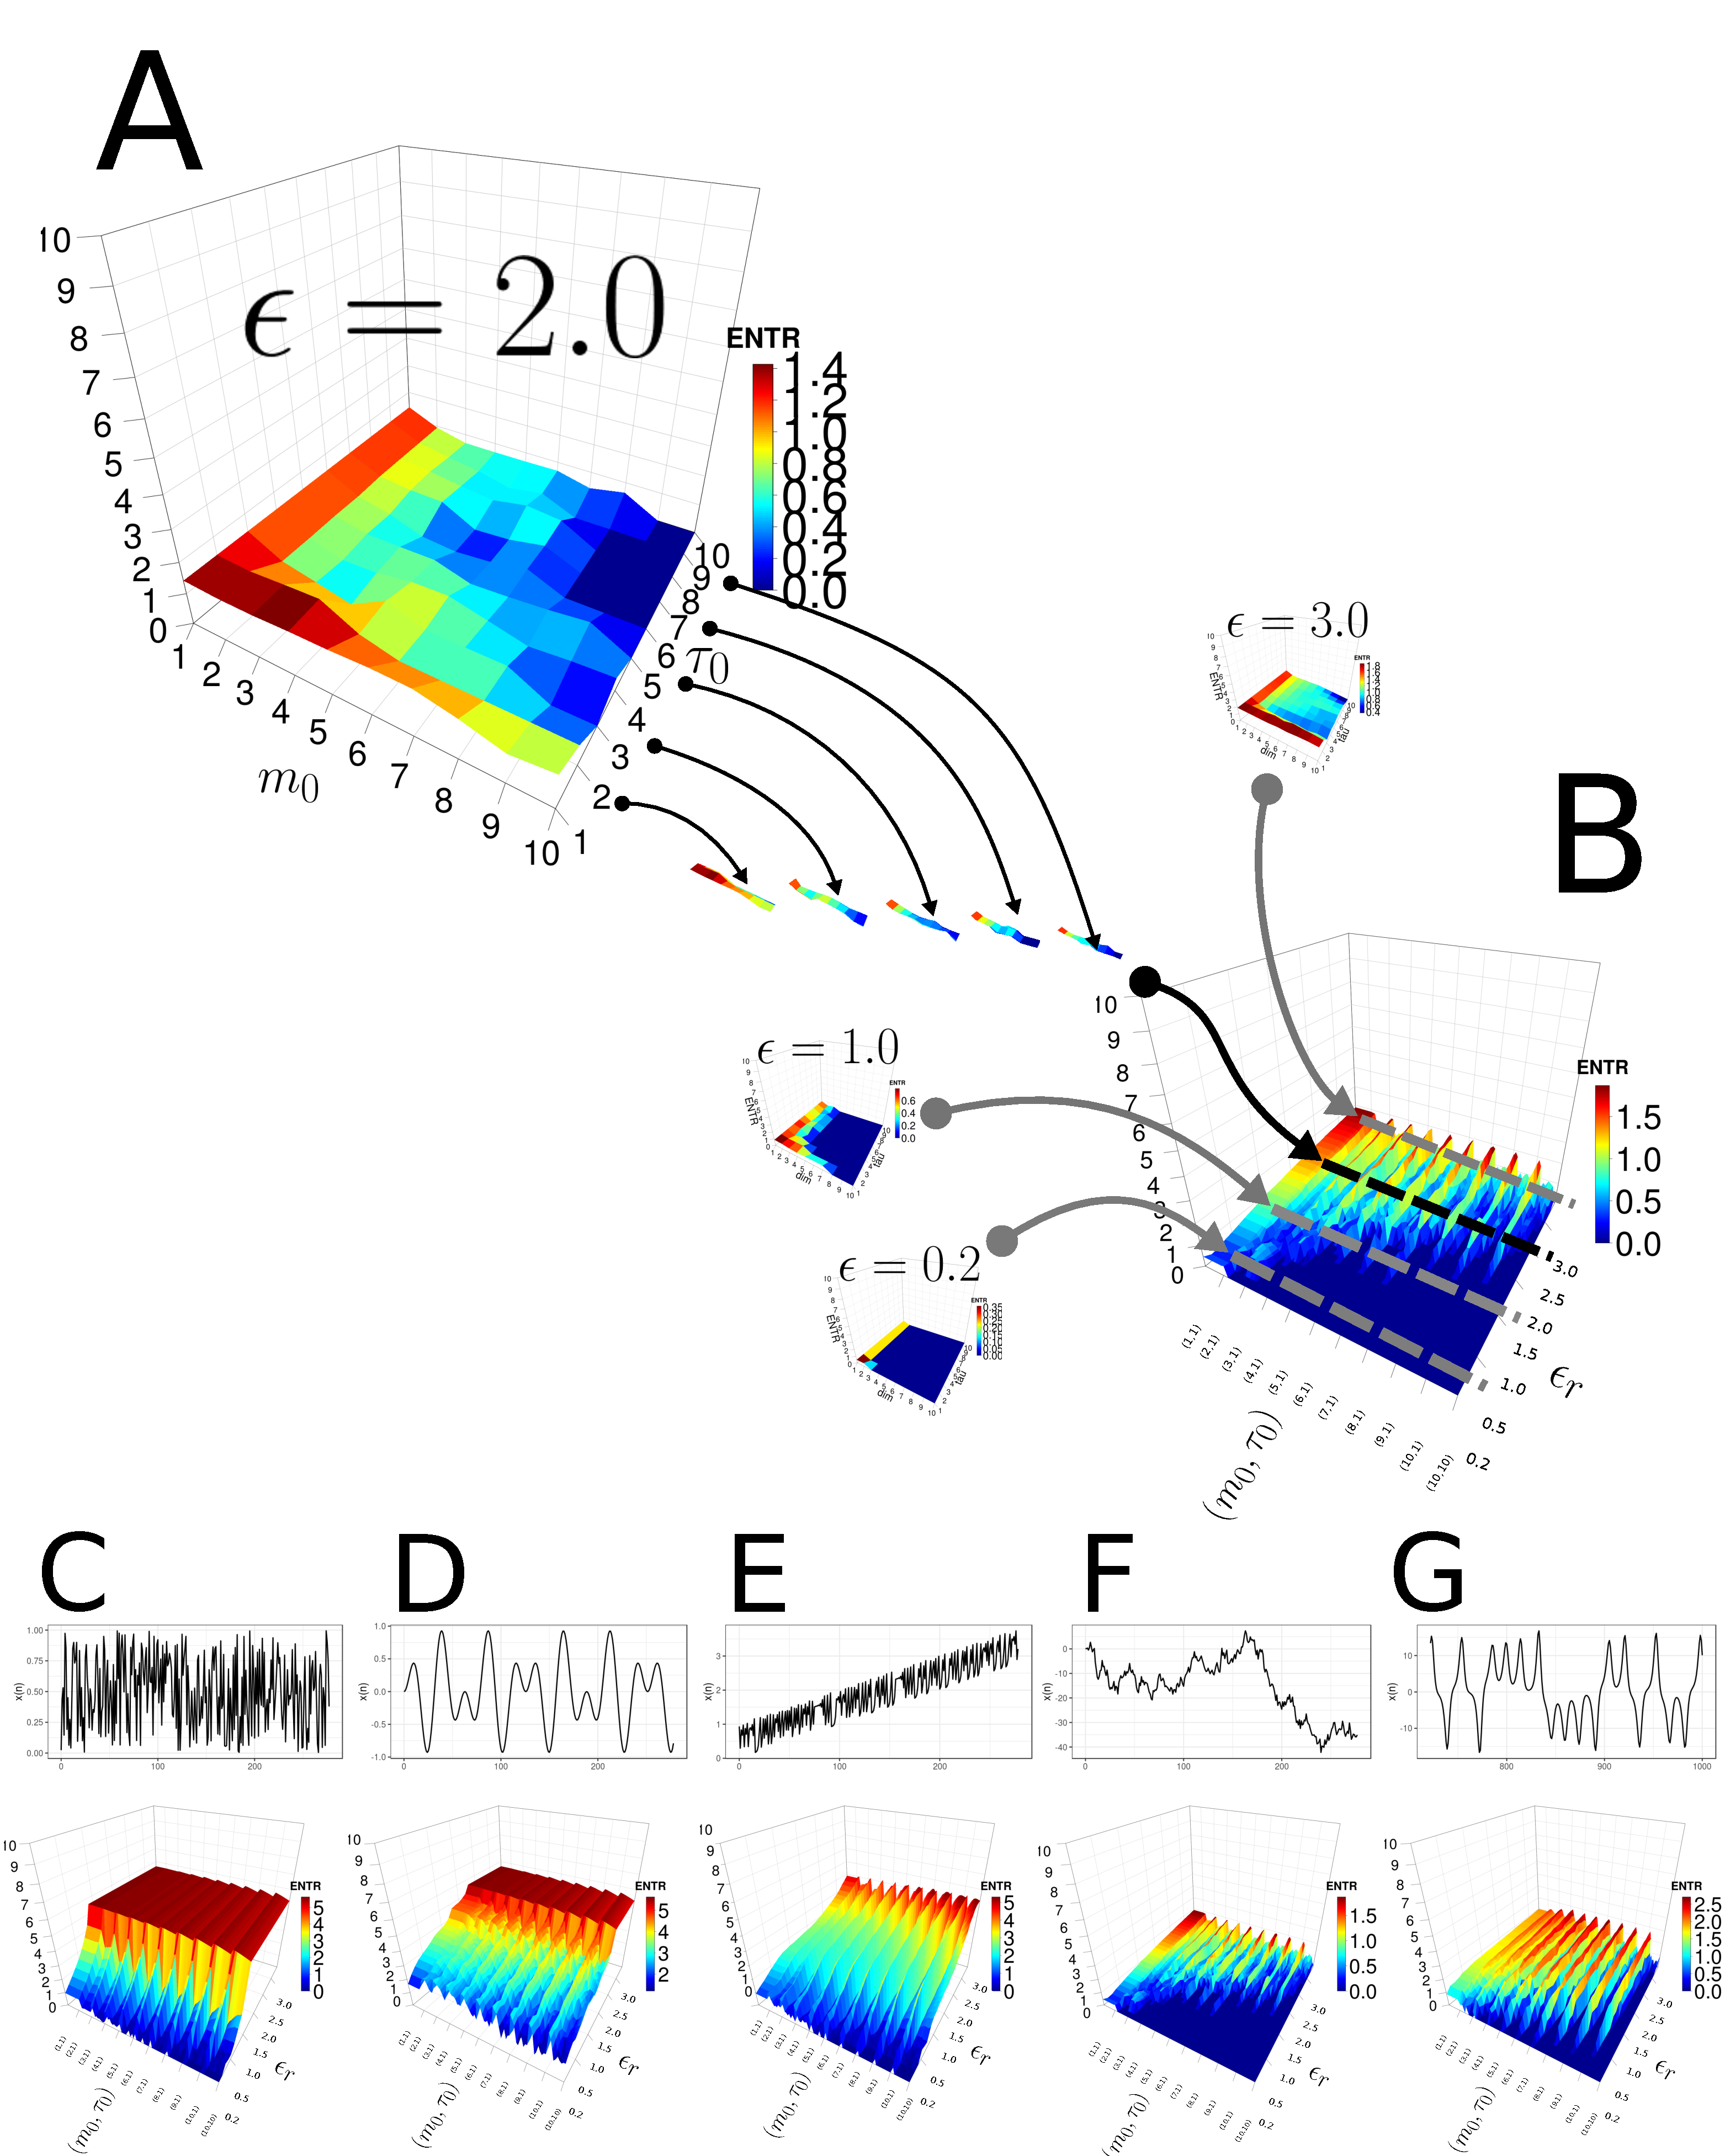
\includegraphics[width=0.95\textwidth]{fig_37}
    \caption
	[3D surface plots]{
	{\bf 3D surface plots.} 
	3D surface plots of RQA ENTR incrementing 
	(A) embedding dimensions ($m$ and $\tau$),
	(B) embedding dimensions ($m$ and $\tau$) and
	recurrence threshold ($\epsilon$).
	Four time-series data and their 3D surface plots of 
	RQA Entr for:
	(C) uniformly distribute noise,
	(D) super-positioned harmonic oscillation 
	($\sin{ \frac{1}{5} t} \sin{ \frac{5}{100}t) }$),
	(E) drift logistic map ($x_{i+1} = 4 x_i (1- x_i) $) corrupted 
	with a linearly increase term ($0.01 i$),
	(F) disrupted brownian motion  ($x_{i+1} = x_i + 2rnorm(1) $), and
	(G) $x(t)$ solution of Lorenz system.
	R code to reproduce the figure is available in \cite{xochicale2018}.
	}
    \label{fig:fig_37}
\end{figure}
%%---------------------------------(FIGURE)-------------------------------------




	\end{verbatim}
	\textit{
	SORTED:  \\
	Mon 29 Apr 02:49:50 BST 2019\\
	Mon 29 Apr 07:05:15 BST 2019
	}
	\\



\end{enumerate}











\end{document}

